% (c) 2012 - 2014 Dimitrios Vrettos - d.vrettos@gmail.com
% (c) 2014 Claudio Carboncini - claudio.carboncini@gmail.com
% (c) 2014 Daniele Zambelli - daniele.zambelli@gmail.com

\chapter{Numeri interi relativi}

\section{I numeri che precedono lo zero}
\label{sec:02_negativi}

Con i numeri naturali non sempre è possibile eseguire l'operazione di 
sottrazione. 
In particolare, non è possibile sottrarre un numero più grande da un numero 
più piccolo, per esempio~$5-12$. 
Tuttavia ci sono situazioni in cui una sottrazione di questo tipo deve essere 
eseguita.

Per esempio, è possibile acquistare un'auto di \officialeuro\ 12\,000 pur avendo 
soltanto risparmi in banca di soli
\officialeuro\ 5\,000. In questo caso si tratta di togliere dai \officialeuro\ 
5\,000 i \officialeuro\ 12\,000 che servono per acquistare
l'auto: materialmente non è possibile e si ricorre a un prestito.

Pensiamo ad una comunicazione dei meteorologi relativa alle previsioni del 
tempo: <<domani la temperatura,
a causa di una perturbazione proveniente dai paesi nordici, potrebbe subire un 
drastico calo e scendere anche di~10 gradi>>. Riflettiamo: se oggi la 
temperatura è di~9 gradi, come possiamo esprimere numericamente la temperatura
prevista per domani? Alcuni diranno: <<il liquido contenuto nel termometro si 
posizionerà al di sotto dello zero>>,
altri <<domani la temperatura sarà di un grado sotto lo zero>> e
altri ancora <<la temperatura sarà di~$-1$ grado>>.

\begin{wrapfloat}{figure}{r}{0pt}
 % (c) 2012 Dimitrios Vrettos - d.vrettos@gmail.com
% Monte Everest e Fossa delle Marianne
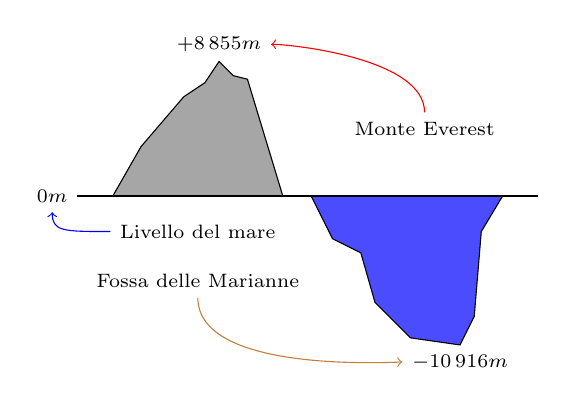
\begin{tikzpicture}[scale=.9]
  % Disegna Everest
  \filldraw[fill=gray!70, draw=black] (0,0)-- (4mm,7mm)-- (10mm,14mm)--(13mm,16mm)-- (15mm,19mm)--(17mm,17mm)--%
	    (19mm,16.5mm)--(24mm,0);
  % Disegna Fossa delle Marianne
  \filldraw[fill=blue!70, draw=black](28mm,0)--(31mm,-6mm)--(35mm,-8mm)--(37mm,-15mm)--(42mm,-20mm)-- (49mm,-21mm)--%
	    (51mm, -17mm)--(52mm, -5mm)--(55mm,0);
  % Disegna il livello del mare 
  \draw[thick] (-5mm,0) -- (60mm,0);

  \begin{scope}[font=\scriptsize]
    % Posiziona altezze
    \node[left] (0)at (-5mm,0) {$0\unit{m}$};
    \node [above](everest) at (15mm,19mm) {$+8\,855\unit{m}$};
    \node [below](marianne) at (49mm,-21mm) {$-10\,916\unit{m}$};
    % Posiziona etichette
    \node (testo1) at (44mm,9.5mm) {Monte Everest};
    \node (testo2) at (12mm,-5mm) {Livello  del mare};
    \node (testo3) at (12mm,-12mm) {Fossa delle Marianne};
  \end{scope}
  % Disegna frecce
  \draw[<-,red ] (everest) .. controls +(right:10mm) and +(up:10mm) .. node[]{} (testo1);
  \draw[<-, blue](0)..controls +(down:5mm) and +(left:19mm)..node[]{} (testo2);
  \draw[<-, brown](marianne)..controls +(left:10mm) and +(down:13mm)..node[]{} (testo3);

\end{tikzpicture}

 \caption{Il monte Everest e la fossa delle Marianne.}
 \label{fig:everest}
\end{wrapfloat}

Leggiamo nel testo di geografia: <<Il punto più profondo della Terra si trova 
nella fossa delle Marianne; esso
supera di~2\,061 metri l'altezza del monte Everest e si trova a~10\,916 metri 
sotto il livello del mare>>.
Se attribuiamo al livello del mare il valore zero, allora potremmo esprimere la 
profondità della Fossa con il
numero~$-10\,916$ e l'altezza del monte Everest con il numero~$+8\,855$ (figura 
\ref{fig:everest}).

Per rappresentare le grandezze che hanno due sensi, come temperature, crediti e 
i debiti, latitudine nord e sud,
altezze sopra il livello del mare e profondità marine i numeri naturali non 
bastano. I matematici in queste
situazioni usano i numeri interi relativi che si scrivono utilizzando gli stessi 
numeri naturali ma preceduti
dal segno~``$+$'' se sono numeri maggiori di~0 e dal segno~``$-$'' se sono 
numeri minori di~0. L'insieme di questi numeri
si costruisce raddoppiando i numeri naturali~$\insN$ e facendo precedere ciascun 
numero dal segno~``$+$'' o~``$-$'',
ad eccezione dello~0, al quale non si attribuisce segno.

\[ \insZ=\lbrace\ldots,-5, -4, -3, -2, -1,~0, +1, +2, +3, +4, +5, \ldots\rbrace 
\]
\newpage

\section{I numeri relativi e la retta}
\label{sec:02_retta}

I numeri relativi possono essere rappresentati su una retta. Disegniamo una 
retta, su di essa prendiamo
un punto di riferimento al quale associamo il numero zero, il verso di 
percorrenza da sinistra verso destra,
un segmento~$AB$ come un'unità di misura. Riportiamo questa unità di misura più 
volte partendo da zero e
procedendo nel verso stabilito aggiungiamo ogni volta uno: ai punti trovati 
associamo gli interi positivi.
Ripetiamo l'operazione partendo dallo zero, ma con il verso di percorrenza a 
sinistra: ai punti trovati associamo
gli interi negativi.

\begin{center}
 % (c) 2012 Dimitrios Vrettos - d.vrettos@gmail.com
% La retta degli interi
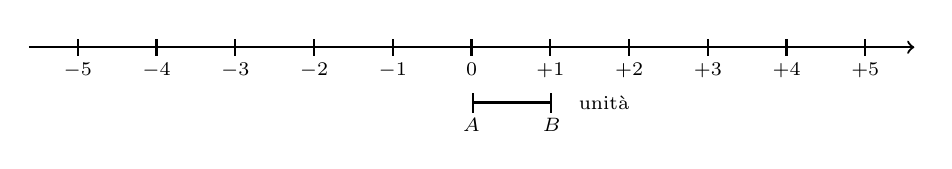
\begin{tikzpicture}
\begin{scope}[thick,font=\scriptsize]
  \draw[->] (-160pt,0)  - -  (160pt,0) node[above]{$\insZ$};	
    \foreach \n in {-5,-4,...,0}{%
      \draw (\n,-3pt) -- (\n,3pt)   node [below=5pt] {$\n$};		
    }

    \foreach \m in {1,2,...,5}{%
      \draw (\m,-3pt) -- (\m,3pt) node [below=5pt]{+$\m$};
    }
  
    \draw[|-|]node [below=22pt]{$A$}(0,-20pt)--(29pt,-20pt) node[below=2pt]{$B$};

    \node [right] at (+35pt,-20pt) {unit\`a};
\end{scope}

\end{tikzpicture}

\end{center}

Possiamo interpretare questi numeri come il numero di passi da fare sulla retta, 
partendo dallo zero verso
destra se il segno è positivo, verso sinistra se il segno è negativo.

L'insieme dei numeri relativi si indica con il simbolo~$\insZ$. In particolare, 
l'insieme dei soli numeri interi relativi
con segno positivo si indica con il simbolo~$\insZ^+$,
l'insieme dei soli numeri interi negativi si indica con il simbolo~$\insZ^-$.

\begin{definizione}
 Due numeri relativi si dicono \emph{concordi}, se hanno lo stesso segno; si 
dicono \emph{discordi} se hanno
 segni opposti.
\end{definizione}

\begin{exrig}
 \begin{esempio}
 Concordi-discordi.
 
$+3$ e~$+5$ sono concordi; \quad 
$+3$ e~$-5$ sono discordi; \quad 
$-5$ e~$-2$ sono concordi.
\end{esempio}
\end{exrig}

\begin{definizione}
Il \emph{valore assoluto} di un numero relativo è il numero senza il segno; 
quindi un numero naturale.
\end{definizione}

Il valore assoluto si indica inserendo il numero relativo tra due barre 
verticali~($\valass{\,}$). In linguaggio
matematico:

\[ \valass{a}=a,\text{ se }a\ge0,\qquad \valass{a}=-a,\text{ se }a<0.\]

\begin{exrig}
 \begin{esempio}
 Valore assoluto.
 
$\valass{+2}=2 \qquad \valass{-5}=5 \qquad 
 \valass{-73}=73 \qquad \valass{+13}=13$
 \end{esempio}
\end{exrig}

\begin{definizione}
 Due numeri interi relativi sono \emph{uguali} se hanno lo stesso segno e lo 
stesso valore assoluto;
 si dicono \emph{opposti} se hanno lo stesso valore assoluto ma segni diversi.
\end{definizione}

Sono numeri opposti~$+3 e -3 \quad +5 e -5 \quad +19 e -19$.

\osservazione Per indicare un numero positivo è possibile scrivere il numero 
senza il segno~``$+$''.
Per esempio si può scrivere indifferentemente~$+1$ o~1,~$+12$ o 
semplicemente~12.

\section{Confronto di numeri relativi}
\label{sec:02_confronto}

Dati due numeri interi relativi quello più grande è quello che sulla retta è 
rappresentato più a destra.
In particolare:
 \begin{enumeratea}
 \item ogni numero intero positivo è maggiore di~0 e di ogni numero negativo;
 \item tra due numeri positivi il più grande è quello che ha valore assoluto 
maggiore;
 \item ogni numero negativo è minore di~0 e di ogni numero positivo;
 \item tra due numeri negativi il più grande è quello che ha valore assoluto 
minore;
 \item 0 è minore di ogni numero positivo e maggiore di ogni numero negativo.
 \end{enumeratea}

Per indicare che un numero è maggiore di un altro si usa separare i due numeri 
con il
simbolo~``$>$''; per indicare che il primo è minore del secondo si usa mettere 
tra i due numeri il simbolo~``$<$''.

\begin{exrig}
 \begin{esempio}
 Confronto di numeri relativi.
 \begin{itemize*}
 \item $+4>+2$: i numeri sono positivi, il maggiore è~$+4$ perché ha valore 
assoluto maggiore;
 \item $-1>-3$: i due numeri sono negativi, il maggiore è~$-1$ perché ha valore 
assoluto minore;
 \item $+4>-2$: il numero positivo è maggiore del numero negativo;
 \item $+4>0$: ogni numero positivo è maggiore di~0;
 \item $0>-2$: ogni numero negativo è minore di~0.
 \end{itemize*}
 \end{esempio}
\end{exrig}

Usando la rappresentazione dei numeri sulla retta l'ordinamento risulta più 
facile da verificare:
il verso di percorrenza della retta (la freccia) indica la direzione nella quale 
i numeri crescono.

% \vspazio\ovalbox{\risolvii \ref{ese:2.1}, \ref{ese:2.2}, \ref{ese:2.3}, 
% \ref{ese:2.4}, \ref{ese:2.5}}

\section{Le operazioni con i numeri relativi}
\label{sec:02_operazioni}

Con i numeri relativi è sempre possibile eseguire le addizioni, le 
moltiplicazioni e le sottrazioni.
Questo significa che se si addizionano, si sottraggono o si moltiplicano due 
numeri relativi il risultato si
trova sempre nella retta dei numeri relativi.

\subsection{Addizione}

Osserviamo prima di tutto che il simbolo di addizione~$(+)$ è lo stesso che si 
usa per indicare il segno dei numeri
positivi, pertanto occorre prestare attenzione quando si incontra il 
segno~``$+$'' al significato che esso ha.
Almeno all'inizio è bene usare una scrittura del tipo~$(+2)+(+5)$ per indicare 
la somma tra i numeri~$+2$ e~$+5$.

L'addizione di due numeri relativi si esegue in due modi diversi a seconda che 
gli addendi siano concordi o discordi.

La \emph{somma di due numeri relativi concordi} è il numero che ha per valore 
assoluto la somma dei singoli valori assoluti e
come segno lo stesso segno degli addendi.
\newpage
\begin{exrig}
 \begin{esempio}
~$(+3)+(+5)=\ldots$: i due numeri da sommare sono concordi, 
il loro segno è~``$+$'', i loro valori assoluti sono~3 e~5,
la loro somma è~8. Pertanto~$(+3)+(+5)=+8$
 \end{esempio}

 \begin{esempio}
~$(-2)+(-5)=\ldots$: i due numeri sono entrambi negativi, quindi sono concordi, 
i loro valori assoluti sono~2 e~5,
la somma ha valore assoluto~7, il segno è~``$-$''. Pertanto
\[(-2)+(-5)=-7.\]
 \end{esempio}

\end{exrig}

La \emph{somma di due numeri relativi discordi} è il numero che ha per valore 
assoluto la differenza dei valori assoluti
e come segno il segno del numero che ha valore assoluto maggiore.

\begin{exrig}
 \begin{esempio}
~$(-5)+(+2)=\ldots$: i due numeri da sommare sono discordi, i loro valori 
assoluti sono~5 e~2, la differenza è~3,
il numero che ha valore assoluto maggiore è~$-5$, pertanto il risultato ha lo 
stesso segno di~$-5$, cioè è negativo.
In definitiva~$(-5)+(+2)=-3$
 \end{esempio}

 \begin{esempio}
~$(+5)+(-2)=\ldots$: i due numeri da sommare sono discordi, i loro valori 
assoluti sono~5 e~2, la loro differenza è~3,
il numero che ha valore assoluto maggiore è~$+5$, pertanto il risultato ha lo 
stesso segno di~$+5$,
cioè è positivo. In definitiva~$(-5)+(-2)=+3$
 \end{esempio}

 \begin{esempio}
~$(+3)+(-7)=\ldots$: i due numeri da sommare sono discordi, i loro valori 
assoluti sono~3 e~7, la loro differenza è~4,
il numero che ha valore assoluto maggiore è~$-7$, quindi il risultato ha segno 
negativo.
In definitiva~$(+3)+(-7)=-4$
 \end{esempio}
\end{exrig}

L'addizione si può rappresentare nella retta dei numeri come l'azione di 
muoversi nel verso indicata dal segno del
secondo addendo: se è positivo si va verso destra, se è negativo si va verso 
sinistra iniziando dal punto che
rappresenta il primo addendo.
 \[(-3)+(+5)=2\]
\begin{center}
 % (c) 2012 Dimitrios Vrettos - d.vrettos@gmail.com

\begin{tikzpicture}[decoration={markings,mark=between positions 0.7 and .9 step 30pt with {\arrow{stealth}}}]
  \begin{scope}[thick,font=\scriptsize]
   \draw[->] (-160pt,0)  - -  (110pt,0) node[above]{$\insZ$};
    \foreach \c in {-3,-2,...,1}{%
     \draw[dotted, color=RedOrange,postaction={decorate}](\c,5pt)--(\c,5pt) arc (180:0:0.5 and 0.5);}
    \foreach \n in {-5,-4,...,0}{%	
     \draw (\n,-3pt) -- (\n,3pt)   node [below=5pt] {$\n$};}
    \foreach \m in {1,2,3}{%	
     \draw (\m,-3pt) -- (\m,3pt)   node [below=5pt] {$+\m$};}

  \end{scope}
 \end{tikzpicture}

\end{center}

\[ (-1)+(-3) = -4\]
\begin{center}
 % (c) 2012 Dimitrios Vrettos - d.vrettos@gmail.com
% Somma -1-3
 \begin{tikzpicture}[decoration={markings,mark=between positions .3 and .5 step 30pt with {\arrowreversed{stealth}}}]
  \begin{scope}[thick,font=\scriptsize]
   \draw[->] (-160pt,0)  - -  (110pt,0) node[above]{$\insZ$};
    \foreach \c in {-4,-3,-2}{%
     \draw[dotted, color=CornflowerBlue,postaction={decorate}](\c,5pt)--(\c,5pt) arc (180:0:0.5 and 0.5);}
    \foreach \n in {-5,-4,...,0}{%	
     \draw (\n,-3pt) -- (\n,3pt)   node [below=5pt] {$\n$};}
    \foreach \m in {1,2,3}{%	
     \draw (\m,-3pt) -- (\m,3pt)   node [below=5pt] {$+\m$};}

  \end{scope}
 \end{tikzpicture}

\end{center}

% \ovalbox{\risolvii \ref{ese:2.6}, \ref{ese:2.7}, \ref{ese:2.8}}
\subsection{Sottrazione}

La sottrazione tra due numeri relativi si esegue facendo la somma del primo 
numero con l'opposto del secondo.

\begin{exrig}
 \begin{esempio}
 Sottrazione di numeri relativi.
 \begin{enumeratea}
 \item $(+2)-(+3)=(+2)+(-3)=-1$
\item $(+1)-(+3)=(+1)+(-3)=-2$
\item $(-2)-(-1)=(-2)+(+1)=-1$
\item $(+3)-(-7)=(+3)+(+7)=+10$
\item $(-5)-(+5)=(-5)+(-5)=-10$
 \end{enumeratea}
 \end{esempio}
\end{exrig}

\begin{inaccessibleblock}[Figura: TODO]
 \begin{figure}[t]
 \centering% (c) 2012 Dimitrios Vrettos - d.vrettos@gmail.com
% Sottrazione 
%
\begin{tikzpicture}
% \begin{scope}[font=\scriptsize]
\matrix [matrix of math nodes,column sep={10mm,between origins}] at (0,0)
{
\node{(+2)};& \node[circle, draw=red](-){-}; & \node[draw=blue,circle] (3pos){(+3)} ;%
& \node{=};& \node{(+2)};& \node[circle, draw=red](+){+};& \node[draw=blue,circle](3neg){(-3)};\\
};


\node (testo1) at (0, -15mm) {Cambio il numero $+3$ con il suo opposto $-3$};
\node (testo2) at (0,15mm) {Cambio la sottrazione in addizione};
% \end{scope}

 \draw[->,red ] (testo2) .. controls +(down:5mm) and +(up:10mm) .. (-) ;
 \draw[->,red ] (testo2) .. controls +(down:5mm) and +(up:10mm) .. (+) ;

 \draw[->,blue ] (testo1) .. controls +(up:10mm) and +(down:10mm) .. (3neg) ;
 \draw[->,blue ] (testo1) .. controls +(up:10mm) and +(down:10mm) .. (3pos) ;

\end{tikzpicture}

 \caption{Esempio~2.9.a.}
\end{figure}
\end{inaccessibleblock}

% \ovalbox{\risolvii \ref{ese:2.9}, \ref{ese:2.10}, \ref{ese:2.11}, 
% \ref{ese:2.12}, \ref{ese:2.13}}

\subsection{Somma algebrica}

Poiché la sottrazione può essere trasformata in addizione, si può semplificare 
la scrittura di addizione
e sottrazione di numeri relativi utilizzando soltanto l'operazione di addizione 
e omettendo di scrivere
il segno~``$+$'' dell'addizione. Questo tipo di addizione tra numeri relativi si 
chiama somma algebrica.

\begin{exrig}
 \begin{esempio}
~$(+1)+(-2)=-1$: se omettiamo il segno di addizione~$(+)$ e le parentesi 
otteniamo~$1-2$.
 \end{esempio}

\begin{esempio}
~$(+1)-(+3)=-2$: si trasforma la sottrazione in addizione con 
l'opposto~$(+1)+(-3)$ omettendo il segno
di addizione~$(+)$ ed eliminando le parentesi si ottiene~$1-3$
 \end{esempio}

\begin{esempio}
~$(-1)+(+2)+(-3)+(+2)+(-7)+(-5)=-12$: si scrive in modo sintetico 
\[-1+2-3+2-7-5.\]
 \end{esempio}

\end{exrig}

La somma algebrica gode delle proprietà associativa e commutativa, pertanto per 
sommare più numeri relativi
si può procedere senza necessariamente rispettare l'ordine in cui sono scritti. 
Per esempio per calcolare
il risultato di~$-1+2-3+2-7-5$ si possono prima sommare tra di loro i numeri 
positivi e~$+2+2=+4$
e poi tra di loro i numeri negativi~$-1-3-7-5=-16$. Quindi~$+4-16=-12$.

% \vspazio\ovalbox{\risolvii \ref{ese:2.14}, \ref{ese:2.15}}

\subsection{Moltiplicazione}

Dati due interi relativi da moltiplicare si chiamano fattori i due numeri e 
prodotto il
risultato dell'operazione.

Il \emph{prodotto di due numeri interi relativi} è il numero intero avente come 
valore assoluto il prodotto
dei valori assoluti dei fattori e come segno il segno~``$+$'' se i fattori sono 
concordi,
il segno~``$-$'' se i fattori sono discordi.

\begin{exrig}
 \begin{esempio}
~$(+3)\cdot(-2)=-6$: il numero~6 si ottiene da~$3\cdot2$, il segno è negativo 
perché i fattori sono discordi.
 \end{esempio}

 \begin{esempio}
~$(-2)\cdot(-3)=+6$: il numero~6 si ottiene da~$3\cdot2$, il segno è positivo 
perché i fattori sono concordi.
 \end{esempio}
 \begin{esempio}
~$(+5)\cdot(+3)=+15$: il numero~15 si ottiene da~$5\cdot3$, il segno è positivo 
perché i fattori sono concordi.
 \end{esempio}
 \begin{esempio}
~$(-1)\cdot(+2)=-2$: il numero~2 si ottiene da~$1\cdot2$, il segno è negativo 
perché i fattori sono discordi.
 \end{esempio}

\end{exrig}

\begin{wrapfloat}{figure}{r}{0pt}
% (c) 2012 Dimitrios Vrettos - d.vrettos@gmail.com
% Moltiplicazione dei segni
\begin{tikzpicture}[font=\Huge]

\matrix (segni) [matrix of nodes]{%
 $\cdot$& $+$ & $-$\\
 $+$& $+$ &$-$\\
 $-$& $-$ &$+$\\
};

  \begin{scope}[thin, blue]
    \draw (segni-2-1.north west)--(segni-2-3.north east);
    \draw (segni-1-2.north west)--(segni-3-2.south west);
  \end{scope}
\end{tikzpicture}

\end{wrapfloat}
Per determinare il segno di un prodotto si può ricorrere alla seguente regola 
dei segni: nella prima riga e
nella prima colonna sono collocati i segni dei fattori, all'incrocio tra la riga 
e la colonna c'è il segno
del risultato.

Nel caso si debbano eseguire più moltiplicazioni il segno del prodotto è 
negativo se il segno meno è presente
in un numero dispari di fattori; se il segno negativo è presente un numero pari 
di volte il prodotto è positivo.

\paragraph{Perché meno per meno fa più; una possibile spiegazione.}
\[0=0\cdot (-2) = (-3+3)\cdot (-2) = (-3)\cdot(-2)+(+3)\cdot(-2)=(-3)(-2)-6.\]

Quale valore dobbiamo assegnare a~$(-3)\cdot(-2)$ affinché il numero ottenuto 
sommato a~$-6$ dia~0?
Evidentemente il numero~$+6$.

\begin{exrig}
 \begin{esempio}
$(+3)\cdot (+2)\cdot (-2) =-12$: \\
il risultato è negativo perché vi è un solo segno~``$-$'' tra i fattori.
 \end{esempio}

 \begin{esempio}
$(-2)\cdot (-3)\cdot (+5)\cdot (-2)\cdot (-1) = +60$: \\ 
il risultato è positivo perché ci sono quattro segni~``$-$''.
 \end{esempio}

 \begin{esempio}
$(-1)\cdot (-2)\cdot (-3)\cdot (-2)\cdot (+2)\cdot (-3) = -72$: \\ 
il risultato è negativo poiché ci sono cinque~``$-$''.
 \end{esempio}
\end{exrig}

% \ovalbox{\risolvii \ref{ese:2.16}, \ref{ese:2.17}, \ref{ese:2.18}}

\subsection{Divisione}

La regola della divisione è del tutto analoga a quella della moltiplicazione.
Per dividere due numeri relativi si dividono i valori assoluti e si attribuisce
al risultato il segno~``$+$'' se i numeri da dividere sono concordi, il 
segno~``$-$'' se i numeri sono discordi.

Osserva che mentre addizione, sottrazione e moltiplicazione sono operazioni 
sempre possibili
tra numeri interi relativi, ossia il risultato di queste operazioni è sempre un 
numero intero
relativo, il risultato della divisione non sempre è un numero intero relativo. 
La divisione
tra numeri relativi è possibile se è possibile la divisione tra i loro valori 
assoluti, ossia se
il divisore è diverso da zero ed è un sottomultiplo del dividendo.
\newpage
\begin{exrig}
 \begin{esempio}
$(+8):(+2)=+4$: \\
il risultato è~4 perché~$8:2=4$, il segno è~``$+$'' perché sono concordi.
 \end{esempio}

\begin{esempio}
$(+9):(-3)=-3$: \\ 
il risultato è~3 perché~$9:3=3$, il segno è~``$-$'' perché sono discordi.
 \end{esempio}

\begin{esempio}
$(-12):(-4)=+3$: \\
il risultato è~3 poiché~$12:4=3$, il segno è~``$+$'' perché sono concordi.
 \end{esempio}

\end{exrig}

% \ovalbox{\risolvii \ref{ese:2.19}, \ref{ese:2.20}, \ref{ese:2.21}}

\subsection{Potenza di un numero relativo}

La definizione di potenza per un numero relativo è la stessa di quella data per 
i numeri naturali
(in questo caso la base è un numero relativo ma l'esponente è un numero 
naturale).
Si moltiplicano tra di loro tanti fattori uguali alla base quante volte è 
indicato dall'esponente.
L'unica attenzione che dobbiamo avere è quella relativa al segno:
 \begin{itemize*}
 \item se la base è un numero positivo il risultato della potenza sarà sempre 
positivo;
 \item se la base è un numero negativo il segno dipende dall'esponente: se 
l'esponente è dispari il
risultato è negativo, se l'esponente è pari il risultato è un numero positivo.
 \end{itemize*}

\begin{exrig}
 \begin{esempio}
 Potenze di numeri relativi.
 \begin{multicols}{2}
 \begin{itemize*}
 \item $(+3)^2=(+3)\cdot(+3)=+9$
 \item $(+3)^3=(+3)\cdot(+3)\cdot(+3)=+27$
 \item $(-2)^2=(-2)\cdot(-2)=+4$
 \item $(-2)^3=(-2)\cdot(-2)\cdot(-2)=-8$
 \item $(-2)^4=+16$
 \item $(-2)^5=-32$
 \item $(-1)^6=+1$
 \item $(-1)^7=-1$
 \end{itemize*}
\end{multicols}
 \end{esempio}

\end{exrig}

Ricordiamo che un qualsiasi numero, diverso da~0, elevato a~0 dà come risultato 
il numero~1 e che qualsiasi
numero elevato a~1 rimane invariato.

\[a^0=1\text{ con }a\neq~0,\qquad a^1=a.\]

 \begin{exrig}
 \begin{esempio}
 Potenze di numeri relativi, con esponente~0 o~1.
\[(-3)^0=1,\qquad (+5)^0=1, \qquad (-2)^1=-2, \qquad (+7)^1=+7 \]
 \end{esempio}

\end{exrig}

% \ovalbox{\risolvii \ref{ese:2.22}, \ref{ese:2.23}, \ref{ese:2.24}, 
% \ref{ese:2.25}, \ref{ese:2.26}, \ref{ese:2.27}}

\subsection{Le proprietà delle operazioni nell'insieme dei numeri relativi}

Le operazioni nei numeri relativi mantengono tutte le proprietà che hanno 
nell'insieme dei numeri naturali, inoltre vale la seguente proprietà:

\subsubsection{Elemento inverso rispetto all'addizione}

Ogni numero intero ha un inverso rispetto all'addizione, cioè per ogni intero 
esiste un altro intero che sommato al primo dà come risultato l'elemento neutro 
dell'addizione:

$a + (-a) = 0; \quad 147 + (-147) = 0$

% Ne numeri relativi valgono tutte le proprietà delle 
% 
% \subsubsection{Proprietà commutativa}
% 
% Un'operazione gode della proprietà commutativa se cambiando l'ordine dei 
% termini il risultato non cambia.
% \paragraph{Somma algebrica}~$a+b=b+a$.
% 
% \emph{Vale} la proprietà commutativa:~$-3+5=5-3=+2$.
% 
% \paragraph{Moltiplicazione}~$a\cdot b=b\cdot a$.
% 
% \emph{Vale} la proprietà commutativa:~$(-3)\cdot(-5)=(-5)\cdot(-3)=+15$.
% 
% \paragraph{Potenza}~$a^b\neq b^a$.
% 
% \emph{Non vale} la proprietà commutativa:~$3^2=9\neq2^3=8$.
% 
% 
% \subsubsection{Proprietà associativa}
% 
% Un'operazione gode della proprietà associativa se presi tre numeri si ottiene 
% sempre
% lo stesso risultato indipendentemente da come si raggruppano i numeri per 
% eseguire l'operazione.
% 
% \paragraph{Somma algebrica}~$(a + b)+c = a+(b+c)$.
% 
% Dovendo sommare~$+3-5-2$ e raggruppando i primi due numeri si ha
% \[(+3-5)-2=-2-2=-4.\]
% Raggruppando gli ultimi due numeri si ha~$3+(-5-2)=3-7 =-4~$.
% 
% Nella somma algebrica tra numeri relativi \emph{vale} la proprietà 
% associativa.
% 
% \paragraph{Moltiplicazione}~$(a \cdot b)\cdot c = a\cdot (b\cdot c)$.
% 
% Dovendo moltiplicare tre o più numeri relativi si può procedere scegliendo a 
% piacere da quale moltiplicazione iniziare. Per esempio,
% dovendo moltiplicare~$(-3)\cdot (-5)\cdot (-2)$,
% si può cominciare dalla prima moltiplicazione~$[(-3)\cdot (-5)]\cdot 
% (-2)=(+15)\cdot (-2)=(-30)$.
% Oppure si può cominciare dalla seconda moltiplicazione~$(-3)\cdot [(-5)\cdot 
% (-2)]=(-3)\cdot (+10)=(-30)$.
% 
% Nella moltiplicazione tra numeri relativi \emph{vale} quindi la proprietà 
% associativa.
% 
% \subsubsection{Elemento neutro}
% 
% Un'operazione su uno specifico insieme numerico ha elemento neutro se esiste, 
% ed è unico, un numero che composto
% con un qualsiasi altro numero lo lascia inalterato.
% 
% Nella somma algebrica l'elemento neutro è~0 sia che si trovi a destra sia che 
% si trovi a sinistra dell'operazione:
% \[+3+0=+3,\qquad -2+0=-2,\qquad~0+5=+5,\qquad~0-4=-4. \]
% 
% Nella moltiplicazione l'elemento neutro è~$+1$ sia a destra sia a sinistra:
% \[-5\cdot (+1) =-5,\qquad +3\cdot (+1) = +3,\qquad +1\cdot (-3) = -3,\qquad 
% +1\cdot (+7) = +7.\]
% 
% Nella divisione l'elemento neutro è~$+1$ solo se si trova a destra:
% \[a:(+1)=a,\qquad +1:a =\ldots. \]
% 
% Dividendo~$+1$ per un numero intero relativo si ottiene un numero intero solo 
% se il divisore è~$+1$ o~$-1$.
% 
% \subsection{Proprietà distributiva della moltiplicazione rispetto 
% all'addizione}
% Moltiplicare il risultato dell'addizione di più numeri per un altro numero dà 
% lo stesso risultato
% che moltiplicare ogni addendo per il fattore e addizionare i prodotti 
% ottenuti. Questa proprietà,
% detta distributiva, vale sia se la somma è a destra sia se è a sinistra.
% \[a\cdot(b+c)=a\cdot b+a\cdot c,\qquad (a+b)\cdot c=a\cdot c+b\cdot c.\]
% 
% \begin{exrig}
%  \begin{esempio}
%  $+3(-2+5)=(+3)(-2)+(+3)(+5)=-6+15=+9$.
% Stesso risultato troviamo se eseguiamo per prima la somma algebrica tra 
% parentesi
% tonda~$(+3)(-2+5)=(+3)(+3)=+9$.
%  \end{esempio}
% 
% \end{exrig}
% 
% \ovalbox{\risolvii \ref{ese:2.28}, \ref{ese:2.29}, \ref{ese:2.30}}

